\documentclass[hidelinks,onefignum,onetabnum,final]{siamart220329}  % for arxiv
%\documentclass[review,hidelinks,onefignum,onetabnum,final]{siamart220329}  % for submission

\usepackage{amsfonts,yhmath}
\usepackage{graphicx}
\usepackage{epstopdf}
\ifpdf
  \DeclareGraphicsExtensions{.eps,.pdf,.png,.jpg}
\else
  \DeclareGraphicsExtensions{.eps}
\fi

% Used for creating new theorem and remark environments
\newsiamremark{remark}{Remark}
\newsiamremark{hypothesis}{Hypothesis}
\crefname{hypothesis}{Hypothesis}{Hypotheses}
\newsiamthm{claim}{Claim}
\newsiamremark{example}{Example}

\usepackage{amsopn}
\DeclareMathOperator{\diag}{diag}

\usepackage{bm,bbm,empheq,verbatim,fancyvrb,amssymb}
\usepackage{booktabs,multirow,xspace}
\usepackage{pifont}

\usepackage{tikz}
\usetikzlibrary{decorations.pathreplacing}
\usetikzlibrary{graphs,quotes}

\newcommand{\eps}{\epsilon}
\newcommand{\RR}{\mathbb{R}}

\newcommand{\grad}{\nabla}
\newcommand{\Div}{\nabla\cdot}

\newcommand{\bbf}{\mathbf{f}}
\newcommand{\bg}{\mathbf{g}}
\newcommand{\bn}{\mathbf{n}}
\newcommand{\bu}{\mathbf{u}}
\newcommand{\bv}{\mathbf{v}}
\newcommand{\bw}{\mathbf{w}}
\newcommand{\bx}{\mathbf{x}}
\newcommand{\bz}{\mathbf{z}}

\newcommand{\bX}{\mathbf{X}}

\newcommand{\bzero}{\bm{0}}

\newcommand{\btau}{\bm{\tau}}

\newcommand{\cB}{\mathcal{B}}
\newcommand{\cH}{\mathcal{H}}
\newcommand{\cK}{\mathcal{K}}
\newcommand{\cV}{\mathcal{V}}

\newcommand{\hcK}{\widehat{\cK}}

\newcommand{\nn}{{\text{n}}}
\newcommand{\pp}{{\text{p}}}
\newcommand{\qq}{{\text{q}}}

\newcommand{\ip}[2]{\left<#1,#2\right>}

\newcommand{\XX}{\ding{55}}

\newcommand{\dx}{\, \mathrm{d}x}

\newcommand{\rhoi}{\rho_{\text{i}}}

\DeclareMathOperator*{\argmin}{arg\,min}
\DeclareMathOperator*{\Hull}{Hull}


% running headers and PDF metadata
\headers{Bounds on geometry errors in glacier simulations}{E. Bueler}

\title{Bounds on geometry errors in glacier simulations}

\author{Ed Bueler\thanks{Department of Mathematics and Statistics, University of Alaska Fairbanks, USA (\email{elbueler@alaska.edu}).}}


\begin{document}
\maketitle

\begin{abstract}
The primary data which determine the evolution of glaciation are bedrock elevation and surface mass balance.  From this data the glacier's geometry solves a free-boundary problem over a set of admissible surface elevation or thickness functions.  This constraint set requires that the ice surface elevation must be above the bedrock topography, equivalently that the ice thickness must be nonnegative.  For implicit time steps the free-boundary problem can be posed in weak form as a variational inequality over a fixed map-plane region.  We conjecture that these continuous-space, implicit time-step problems must be well-posed in the case of Stokes dynamics.  Then we show an abstract estimate for finite element approximations of variational inequality problems over Banach spaces, in which the nonlinear operator is assumed to be coercive and Lipshitz.  When applied in the glacier case, all terms can be interpreted and further estimated.  The resulting computable bounds on the geometry approximation error are demonstrated in an implicit time-stepping glacier simulation based on non-shallow Stokes dynamics.
\end{abstract}

% REQUIRED
\begin{keywords}
error bounds, finite element methods, glaciers, ice flow, variational inequalities
\end{keywords}

% REQUIRED
%\begin{MSCcodes}
%FIXME
%\end{MSCcodes}


\section{Introduction} \label{sec:intro}

Glacier and ice sheet simulations typically model the ice layer as a free-surface, very-viscous, incompressible, and non-Newtonian fluid \cite{GreveBlatter2009,SchoofHewitt2013}.  For simplicity we will restrict our considerations to simulations of glaciers on land, without floating portions, and we note that an ``ice sheet'' is simply a continent-scale glacier.  Two types of essential input data into such simulations are the bedrock elevation and the surface mass balance (SMB).  We will assume that the bedrock elevations are constant in time.  By definition, the SMB is the annually-averaged difference of vertically-accumulating snow minus the loss of (liquid) water, through runoff, at the upper surface of the glacier \cite{Cogleyetal2011}.  Note that elevations are measured here in meters, and that SMB is measured in ice-equivalent units of meters per second.

Thus a glacier simulation takes initial glacier geometry, the bedrock topography, and the time-dependent climate as inputs.  It produces the glacier's evolving geometry and flow velocity; these are the output fields of primary scientific value.  The geometry is parameterized by a surface elevation or thickness function; these depend on map-plane (two-dimensional) location and time.  The computed flow velocity is, however, only defined at those three-dimensional locations and times where ice is present.

Additional complications are common in comprehensive models \cite{GreveBlatter2009}, including simulation of the internal energy of the ice \cite{Aschwandenetal2012}, and/or the presence of liquid water within the ice matrix or at the glacier surfaces.  However, here we consider only models which conserve mass and momentum, and which do not make shallowness assumptions.  Conservation of energy is not addressed.

At a map-plane location and time where a glacier exists the surface elevation exceeds the bedrock elevation, equivalently the ice thickness is positive.  In other words, however parameterized, the glacier's geometry must satisfy an inequality so as to be admissible.  In fact, let $\Omega \subset \RR^2$ be a fixed portion of the earth's surface on which we are interested in glaciation (Figure \ref{fig:stokesdomain}).  Let $x\in\Omega$ denote the map-plane coordinate(s).  Assume we are given, as data, a bed elevation function $b(x)$ and an SMB function $a(t,x)$ for $t\in [0,T]$ and $x\in \Omega$.  (Function spaces for these data will be considered below.)  Noting that $a$ is generally signed, in areas where $a>0$ (accumulation; draw as downward arrows in Figure \ref{fig:stokesdomain}) then a glacier will exist, but if $a<0$ (upward arrows) then either a glacier exists with an ablating surface, or no glacier exists.  Determining which situation applies at a given $x\in\Omega$ requires solving a free-boundary problem.

\medskip
\begin{figure}[ht]
\centering
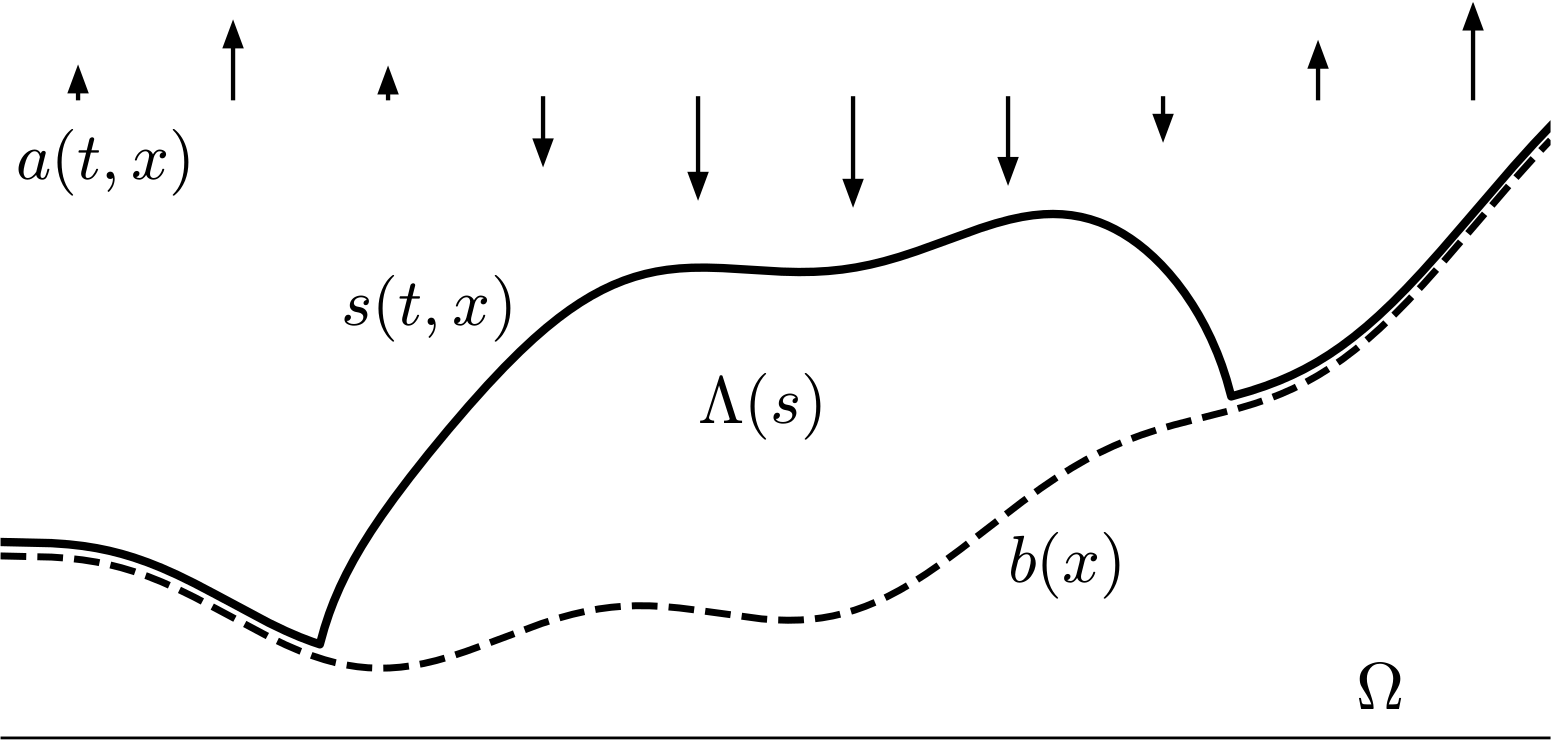
\includegraphics[width=0.65\textwidth]{genfigs/stokesdomain.pdf}
\caption{Glacier geometry notation used in this paper.}
\label{fig:stokesdomain}
\end{figure}

\medskip
Let $s(t,x)$ be the (solution) ice surface elevation.  We will regard this as defined everywhere, but subject to the constraint that the surface $z=s(t,x)$ must be at or above the bedrock, $s(t,x) \ge b(x)$, though some regions in $\Omega$ may have no ice $s(t,x)=b(x)$.  The solution ice velocity $\bu(t,x,z)$ and pressure $p(t,x,z)$ are then defined only on the 3D domain
\begin{equation}
\Lambda(t) = \left\{(x,z)\,:\,b(x) < z < s(t,x)\right\} \subset \Omega \times \RR. \label{eq:icydomain}
\end{equation}
This aspect of glacier modeling deserves emphasis: at any time $t$ the 3D domain $\Lambda(t)$, on which the velocity and pressure are meaningful, is determined by the time-dependent surface elevation $s(t,x)$, which is also part of the solution.

Denote the surface value (trace \cite{Evans2010}) of the velocity solution by $\bu|_s$, and let $\bn_s = \left<-\grad s,1\right>$ be a 3D, un-normalized surface normal vector.  For any $T>0$, an infinite-dimensional nonlinear complementarity problem (NCP) \cite{Bueler2021conservation,FacchineiPang2003,SchoofHewitt2013} applies almost everywhere in $[0,T]\times \Omega$:
\begin{subequations}
\label{eq:ncp}
\begin{align}
s - b &\ge 0 \\
\frac{\partial s}{\partial t} - \bu|_s \cdot \bn_s - a &\ge 0 \\
(s - b) \left(\frac{\partial s}{\partial t} - \bu|_s \cdot \bn_s - a\right) &= 0
\end{align}
\end{subequations}
This strong form NCP statement, which will be reformulated as a variational inequality (VI; \cite{KinderlehrerStampacchia1980}) in Section \ref{sec:models}, assumes the extension $\bu|_s=0$  to the ice-free areas where $s(t,x)=b(x)$.  This NCP says that either a location is ice free ($s-b=0$) or the surface kinematical equation (SKE) holds:
\begin{equation}
\frac{\partial s}{\partial t} - \bu|_s \cdot \bn_s - a = 0.  \label{eq:ske}
\end{equation}

Well-known equation \eqref{eq:ske} states that the (non-material) surface of the ice moves vertically according to the sum of a component of the ice velocity at the surface and the SMB \cite{SchoofHewitt2013}.  This is a statement of mass conservation at a non-material surface \cite{Aschwandenetal2012}, sometimes wrongly\footnote{Equation \eqref{eq:ske} is not the boundary condition for any identifiable problem.} called a ``kinematical boundary condition'' \cite{GreveBlatter2009}.

Within the ice the simulation will conserve mass and momentum.  Recalling \eqref{eq:icydomain}, let $\Gamma_s(t) \subset \partial \Lambda(t)$ be the upper surface $z=s$ and
$\Gamma_b(t) \subset \partial \Lambda(t)$ be the base $z=b$.  The models considered here neglect the possibility of fracture-generated cliffs at the ice margin, and we assume $\partial \Lambda(t) = \Gamma_s(t) \cup \Gamma_b(t)$ at any time.

The standard non-shallow model is then a non-Newtonian Stokes problem \cite{GreveBlatter2009,JouvetRappaz2011,SchoofHewitt2013} over $\Lambda(t)$.  If $D\bu=\frac{1}{2}(\grad \bu + \grad \bu^{\top})$ denotes the strain rate tensor then the formula
\begin{equation}
\nu(D\bu) = \frac{\Gamma}{2} |D\bu|^{\pp-2} \label{eq:glen}
\end{equation}
defines the shear-thinning ice viscosity according to Glen's power law \cite{GreveBlatter2009}.  The exponent $\pp$, often written $\pp=(1/\nn)+1$ in glaciology \cite{GoldsbyKohlstedt2001}, is approximately 4/3; note $\pp=2$ yields a Newtonian fluid.  The coefficient $\Gamma>0$ is determined by the measured properties of ice \cite{GoldsbyKohlstedt2001,GreveBlatter2009}, but we assume it to be constant, modeling an isothermal situation.  If $\rhoi$ is the density of ice and $\bg$ is the acceleration of gravity then a glacier with nonsliding (e.g.~frozen) base \cite{JouvetRappaz2011} has velocity and pressure solving the following equations:
\begin{subequations}
\label{eq:stokes}
\begin{align}
- \nabla \cdot \left(2 \nu(D\bu)\, D\bu\right) + \nabla p &= \rhoi \bg && \text{within $\Lambda(t) \subset \RR^3$} \\
\nabla \cdot \bu &= 0 && \text{within $\Lambda(t) \subset \RR^3$} \label{eq:stokes:incomp} \\
\left(2 \nu(D\bu) D\bu - pI\right) \bn_s &= \bzero && \text{on $\Gamma_s(t)$}\label{eq:stokes:stressfreesurface} \\
\bu  &= \bzero && \text{on $\Gamma_b(t)$}
\end{align}
\end{subequations}
Equation \eqref{eq:stokes:incomp} states incompressibility.  Boundary condition \eqref{eq:stokes:stressfreesurface} says that the sub-aerial upper surface is stress free; it should not be confused with \eqref{eq:ske}.

In summary at this point, a glacier simulation is an evolving free-surface flow, subject to a signed climate that can add or remove ice, coupled to a Stokes problem within an evolving, 3D icy domain.  The evolution of the solution variables $s(t,x)$, $\bu(t,x,z)$, and $p(t,x,z)$ is found from an initial surface elevation $s(0,x)$ and the data $b(x),a(t,x)$.  The surface elevation $s(t,x)$ is defined everywhere over $[0,T]\times \Omega$, but it is subject to $s(t,x) \ge b(x)$.

The surface elevation $s(t,x)$ and surface velocity $\bu|_s(t,x)=\bu(t,x,s(t,x))$ are linked by the kinematical NCP \eqref{eq:ncp}.  However, the Stokes model \eqref{eq:stokes} acts as an instantaneous ``algebraic'' constraint on the evolution statement \eqref{eq:ncp}; it acts instantaneously because the flow is very viscous \cite{Acheson1990}.  The coupled, infinite-dimensional problem \eqref{eq:icydomain}--\eqref{eq:stokes} is therefore both a differential algebraic equation (DAE) system \cite{AscherPetzold1998} and an NCP.

Glacier simulations are commonly formulated using a finite element (FE) method for the Stokes sub-problem \cite{IsaacStadlerGhattas2015,Jouvetetal2008,Pattynetal2008}, or for a shallow approximation thereof.  To the author's knowledge all existing non-shallow (Stokes) evolution models use a explicit time-stepping scheme for the geometry, for example as in \cite{Jouvetetal2008} or \cite{LofgrenAhlkronaHelanow2022}, with the one exception of the work \cite{WirbelJarosch2020}.  By contrast, each time step of an implicit-stepping model will solve a variational inequality (VI) weak formulation \cite{Evans2010,KinderlehrerStampacchia1980}.  We must choose whether glacier geometry in this formulation is parameterized by surface elevation or thickness.  While equivalent in the continuum problem, the two formulations have different character when FE approximations are applied.  For this work, including the abstract estimate of Section \ref{sec:abstractestimate}, surface elevation $s(t,x)$ is preferred because of the flow-caused smoothing effect illustrated in Figure \ref{fig:giscross}.  For land-based glaciers $s(t,x)$ is smoother in $x$ than is the thickness $H(t,x) = s(t,x)-b(x)$ because the latter ``inherits'' the lower regularity of the eroded and faulted bedrock topography.

\begin{figure}
\begin{minipage}[t]{0.85\textwidth}
\vspace{0pt}
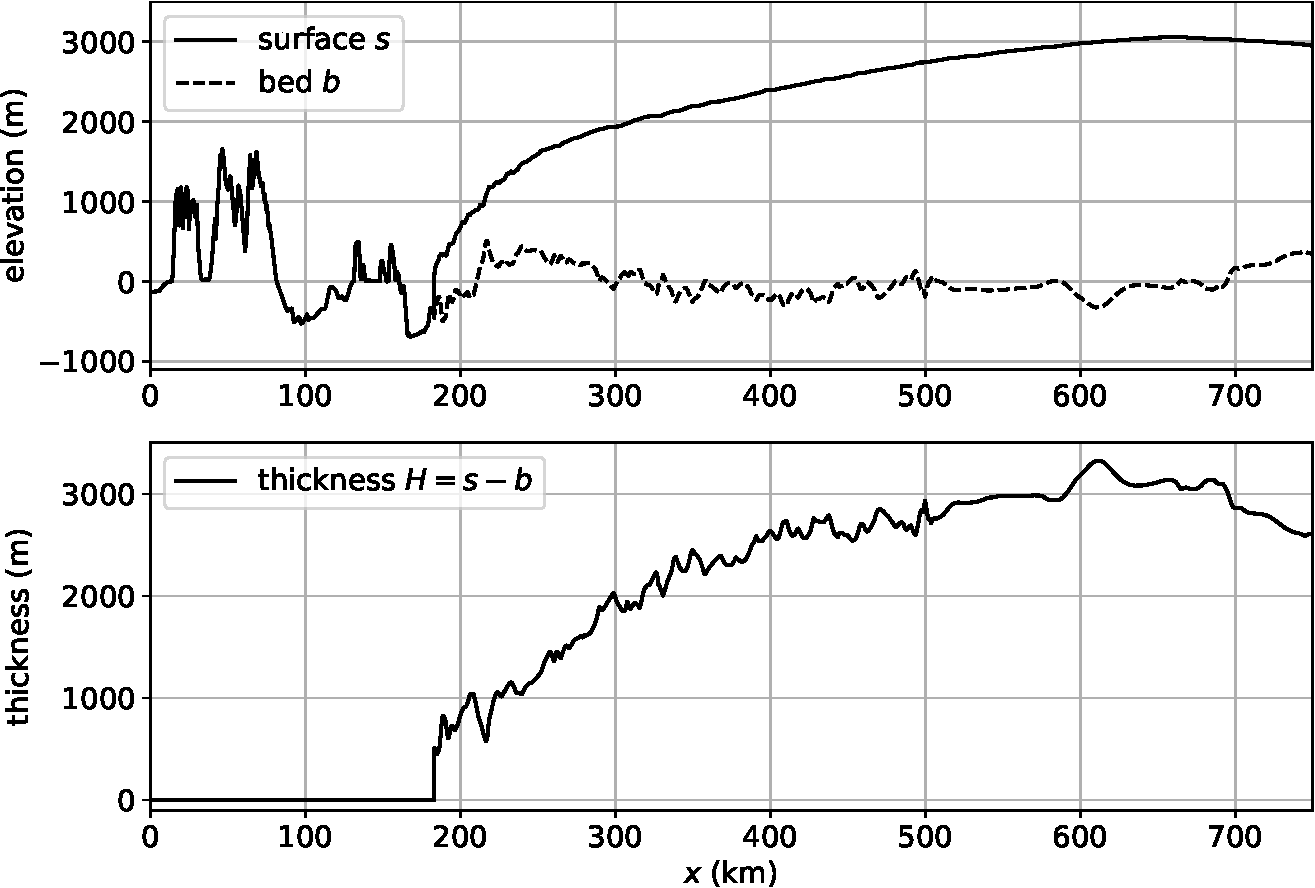
\includegraphics[width=\textwidth]{genfigs/giscross.pdf}
\end{minipage}
\,
\begin{minipage}[t]{0.13\textwidth}
\vspace{10pt}
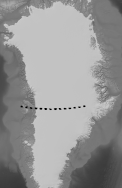
\includegraphics[width=\textwidth]{genfigs/gis/gris-profile-gray.png}
\end{minipage}
\caption{A cross-section of the Greenland ice sheet at $70^\circ$N latitude (inset).  While the ice surface $s$ is relatively smooth because of ice flow (top), the bedrock elevation $b$ is much rougher.  The corresponding ice thickness $H = s-b$ (bottom), though it is a valid description of glacier geometry, inherits the low regularity of $b$.  (Data from \cite{Morlighemetal2017} and A.~Aschwanden, personal communication.)}
\label{fig:giscross}
\end{figure}

FIXME: WHAT WE ACCOMPLISH

This paper is organized as follows.  In Section \ref{sec:models} we reformulate the coupled problem \eqref{eq:icydomain}--\eqref{eq:stokes} as a VI weak form for (implicit) backward Euler time steps.  Well-posedness for this time-step problem is conjectured over a Banach space of surface elevation functions.  Then in Section \ref{sec:abstractestimate} we show an abstract FE error estimate (Theorem \ref{thm:abstractestimate} and its corollaries) for general VI problems involving fully-nonlinear, but coercive and Lipshitz, operators on Banach spaces.  This estimate extends the classical bilinear, elliptic case by Falk \cite{Falk1974}.  In Section \ref{sec:application} we apply this theorem to the glacier time steps from Section \ref{sec:models}.  The distinctive character of how glaciers respond to climate implies that certain terms are effectively small, and so a computable geometry error upper bound follows.  The estimate is demonstrated in Section \ref{sec:demo} on an idealized, but non-trivial, glacier simulation implemented in Firedrake \cite{Hametal2023}.


\section{Implicit time-stepping weak-form models} \label{sec:models}

In the following time-stepping model, the SMB $a(t,x)$ is assumed to be defined everywhere in $\Omega$, regardless of whether a glacier is present or not.  At an ablative location the value $a(t,x)\le 0$ can be modeled using precipitation and an energy balance \cite{GreveBlatter2009}, for instance by hypothesizing an ice or snow surface and then computing the total runoff from the available energy for melt, balanced against snow accumulation, if any.  Thus $a(t,x)$ at an unglaciated location will be the SMB which a glacier would experience if it were present at that time and place.

Let $\{t_n\}$ be an increasing sequence of times, and denote $\Delta t = t_n-t_{n-1}$ for a generic time step.  Write $s^n(x)\approx s(t_n,x)$ for the unknown surface elevation at time $t_n$.  Using a backward Euler implicit step \cite{AscherPetzold1998}, SKE \eqref{eq:ske} is approximated by
\begin{equation}
\frac{s^n - s^{n-1}}{\Delta t} - \bu|_{s^n} \cdot \bn_{s^n} - a^n = 0. \label{eq:be:ske}
\end{equation}
Here $a^n$ is the temporal average of $a(t,x)$ over $[t_{n-1},t_n]$, so define the source term
\begin{equation}
\ell^n(x) = s^{n-1}(x) + \int_{t_{n-1}}^{t_n} a(t,x)\,dt, \label{eq:be:source}
\end{equation}
such that $\ell^n=s^{n-1}+\Delta t\,a^n$.

The implicit step solution $s^n$, denoted from now on simply by $s$, does not solve \eqref{eq:be:ske} over all of $\Omega$.  Instead, similar to \eqref{eq:ncp}, the updated surface solves an NCP:
\begin{subequations}
\label{eq:be:ncp}
\begin{align}
s - b &\ge 0 \label{eq:be:ncp:constraint} \\
s - \Delta t\,\bu|_s \cdot \bn_s - \ell^n &\ge 0 \\
(s - b) \left(s - \Delta t\,\bu|_s \cdot \bn_s - \ell^n\right) &= 0 \label{eq:be:ncp:complementarity}
\end{align}
\end{subequations}
Equation \eqref{eq:be:ncp:complementarity} says that either there is no ice ($s=b$) or the SKE \eqref{eq:be:ske} holds, almost everywhere.

The strong form NCP \eqref{eq:be:ncp} has a weak form VI version which is suited to finite element (FE) approximation.  The precise Banach space $\cV$ of surface elevations in this VI is unknown; this is addressed later in the Section.  Admissible surface elevations are from a convex and closed subset of $\cV$:
\begin{equation}
\cK = \left\{r \in\cV\,:\,r \ge b\right\}.  \label{eq:be:admissible}
\end{equation}
Then the following argument derives the VI form \cite{Bueler2021conservation}.  Suppose $s$ is continuous and sufficiently-regular to solve NCP \eqref{eq:be:ncp}.  Let $\Omega_I$ be a measurable subset of $\Omega$ on which constraint \eqref{eq:be:ncp:constraint} is inactive, so a glacier is present: $\Omega_I \subset \{x\,:\,s(x)>b(x)\}$.  Because \eqref{eq:be:ske} holds on $\Omega_I$ it follows by integration that
\begin{equation}
\int_{\Omega_I} \left(s - \Delta t\,\bu|_s \cdot \bn_s - \ell^n\right)\,(r-s) = 0.  \label{eq:inactivetruth}
\end{equation}
for all $r\in\cK$.  On the other hand, suppose $\Omega_A \subset \{x\,:\,s(x)=b(x)\} \subset \Omega$ is a measurable subset of the active (ice-free) region.  Note that $r-s=r-b\ge 0$ on $\Omega_A$ for $r\in\cK$, and observe that $\ell^n - b \le 0$ on all of $\Omega_A$ because otherwise, using the continuity of $b$, $s^{n-1}$, and $a^n$, a glacier would still be present or would have appeared somewhere in $\Omega_A$, a contradiction.  Using $\bu|_s=0$ on $\Omega_A$, i.e.~extension by zero, integration yields an inequality because $b-\ell^n \ge 0$ and $r-s\ge 0$ on $\Omega_A$:
\begin{equation}
\int_{\Omega_A} \left(s - \Delta t\,\bu|_s \cdot \bn_s - \ell^n\right)\,(r-s) = \int_A \left(b - \ell^n\right)\,(r-b) \ge 0.  \label{eq:activetruth}
\end{equation}
All parts of $\Omega$ are either covered by glacier (in some $\Omega_I$) or ice free (in $\Omega_A$), almost everywhere, so addition of \eqref{eq:inactivetruth} and \eqref{eq:activetruth} justifies the following VI model for $s \in \cK$:
\begin{equation}
\int_\Omega \left(s - \Delta t\,\bu|_s \cdot \bn_s\right)\,(r-s) \ge \int_\Omega \ell^n \,(r-s) \quad \text{for all } r \in \cK. \label{eq:be:viearly}
\end{equation}
	
We also need the weak form of the Stokes equations on $\Lambda(t)$; recall definition \eqref{eq:icydomain}.  The Stokes problem computes $\bu|_s$ where it appears in VI \eqref{eq:be:viearly}.

Suppose temporarily that $\Lambda = \Lambda(t) \subset \RR^3$ is a fixed, bounded domain.  Denote by $W^{k,r}(\Lambda)$ the Sobolev space \cite{Evans2010} of functions with $k$ weak derivatives which are $r$th-power integrable.  We will assume that the ice base $\Gamma_b\subset\partial \Lambda$, on which we prescribe a Dirchlet condition $\bu=\bzero$, has positive measure, but otherwise we suppose that the boundary $\partial \Lambda$ is stress-free.  Recall from the Introduction that $\pp=(1/\nn)+1\approx 4/3$.  Let $W_0^{1,\pp}(\Lambda)^{3}$ be the space of velocity functions, zero along $\Gamma_b$, and let
\begin{equation}
\mathcal{M}_\Lambda = W_0^{1,\pp}(\Lambda)^3 \times L^\qq(\Lambda)  \label{eq:mixed}
\end{equation}
be the (mixed) space of admissible velocity and pressure pairs.  The Glen-Stokes solution $(\bu,p) \in \mathcal{M}_\Lambda$ satisfies the weak form
\begin{equation}
F_\Lambda(\bu,p)[\bv,q] = \int_\Lambda 2 \nu(|D\bu|) D\bu : D\bv - p \Div\bv - (\Div\bu) q - \rhoi \bg \cdot \bv = 0 \label{eq:glenstokesweak}
\end{equation}
for all $(\bv,q) \in \mathcal{M}_\Lambda$.

Jouvet and Rappaz \cite{JouvetRappaz2011} prove that \eqref{eq:glenstokesweak} is well-posed under the above assumptions if also the Neumann boundary of $\Lambda$ is $C^1$; we return to this regularity concern below.  They show well-posedness via the equivalence of \eqref{eq:glenstokesweak} and minimization of a convex and coercive functional over the divergence-free subspace.  Observe that if the solution is sufficiently regular then it satisfies strong equations \eqref{eq:stokes}.

The well-posedness of weak-form problem \eqref{eq:glenstokesweak} allows us to create a well-defined map from the surface $s=s^n$ to the surface value of the velocity solution $\bu=\bu^n$ .  The map is defined via definition \eqref{eq:icydomain} of $\Lambda(t_n)$, the solution of \eqref{eq:glenstokesweak} over that domain, and then evaluation of the trace of $\bu$ over $\Gamma_N\subset \partial\Lambda$.  Concretely we define
\begin{equation}
\Phi(s) = - \bu|_s\cdot \bn_s, \qquad \Phi:\cV \to \cV', \label{eq:be:Phidefine}
\end{equation}
as the \emph{surface motion map}.  For any surface elevation $s$, this map evaluates the term in the SKE \eqref{eq:be:ske} which arises from solving the conservation of momentum problem \eqref{eq:glenstokesweak}.  Therefore, recalling NCP \eqref{eq:be:ncp}, we define the weak form operator
\begin{equation}
F_{\Omega,\Delta t}(s)[r] = \Delta t\,\Phi(s)[r] + \int_\Omega s r = \int_\Omega \left(s - \Delta t\, \bu|_s \cdot \bn_s\right) r.  \label{eq:be:Fdefine}
\end{equation}

VI problem \eqref{eq:be:viearly} can now be written using well-defined maps, as long as the solution surface elevations $s$ are sufficiently-regular so that the corresponding Stokes problems are well-posed.  Observing that the source term $\ell^n$, defined in \eqref{eq:be:source}, provides an element of the dual space $\cV'$, we seek $s = s^n \in \cK$ so that
\begin{equation}
\ip{F_{\Omega,\Delta t}(s)}{r-s} \ge \ip{\ell^n}{r-s} \quad \text{for all } r \in \cK. \label{eq:be:vi}
\end{equation}
This is the abstract weak form associated to strong form \eqref{eq:be:ncp}.

FIXME conjecture well-posedness of \eqref{eq:be:vi} for sufficiently short $\Delta t$

FIXME compare VI for mass continuity with $H$: fluid layer thickness equation, also called mass continuity or Saint Venant equation \cite{JouvetBueler2012}, $\cK = \{H\ge 0\}$, $\cK_h \subset \cK$, apparently $\eta = H^{2p/(p-1)} \in W^{1,p}(\Omega)$, for e.g.~$p=4$, because of existence in SIA case \cite{JouvetBueler2012}; SIA model has better-known properties \cite{JouvetBueler2012,PiersantiTemam2023}. however, regularity arising from analyzing SIA is not to be trusted because non-shallow (Stokes) dynamics is not diffusive for short wavelength surface/thickness perturbations \cite{Pattynetal2008}


\section{Abstract error estimate} \label{sec:abstractestimate}

We consider an abstract variational inequality (VI) \cite{KinderlehrerStampacchia1980} problem as follows.  Let $\cV$ be a real reflexive Banach space with norm $\|\cdot\|$ and topological dual space $\cV'$.  Denote the dual pairing of $\phi \in \cV'$ and $v\in\cV$ by $\ip{\phi}{v} = \phi(v)$, and define the (Banach space) norm on $\cV'$ by $\|\phi\|_{\cV'} = \sup_{\|v\|=1} |\!\ip{\phi}{v}\!|$.  Let $\cK \subset \cV$ be a nonempty, closed, and convex subset, the constraint set; elements are said to be admissible.  For a continuous, but generally nonlinear, operator $f:\cK \to \cV'$, and a linear source $\ell\in \cV'$, the VI problem is to find $u\in \cK$ such that
\begin{equation}
\ip{f(u)}{v-u} \ge \ip{\ell}{v-u} \quad \text{for all } v\in \cK. \label{eq:vi}
\end{equation}
The best know example of \eqref{eq:vi} is the obstacle problem for the Laplacian operator; see e.g.~subsections 8.4.2 in \cite{Evans2010}, and subsection 5.1 in \cite{Ciarlet2002} for its FE analysis.

\begin{definition} \label{def:monotonepcoercive}
An operator $f:\cK \to \cV'$ is said to be \emph{monotone} if
\begin{equation}
\ip{f(v)-f(w)}{v-w} \ge 0 \qquad \text{for all } v,w \in \cK \label{eq:monotone}
\end{equation}
and \emph{strictly monotone} if equality in \eqref{eq:monotone} implies $v=w$.  Let $p>1$.  The operator is \emph{$p$-coercive} \cite{Bueler2021conservation} if there exists $\alpha>0$ such that
\begin{equation}
\ip{f(v)-f(w)}{v-w} \ge \alpha \|v-w\|^p \qquad \text{for all } v,w \in \cK. \label{eq:pcoercive}
\end{equation}
\end{definition}

Clearly, if $f$ is $p$-coercive then it is monotone and strictly monotone, in which case any solution of \eqref{eq:vi} is unique.  Furthermore, it is well-known that if $f:\cK \to \cV'$ is also continuous on finite-dimensional subspaces then VI \eqref{eq:vi} has a solution \cite[Corollary III.1.8]{KinderlehrerStampacchia1980}.  Thus $p$-coercivity and appropriate continuity of $f$ show well-posedness for \eqref{eq:vi}.

% \cite{Peral1997} uniform continuity over bounded sets for p-Laplacian: Thm A.0.6

\begin{definition} \label{def:lipshitz}
For $\rho>0$ let $B_\rho = \{v\in \cV\,:\,\|v\|\le \rho\}$.  We say $f:\cK \to \cV'$ is \emph{Lipshitz on bounded sets of $\cK$} if for every $\rho>0$ there is $C(\rho)>0$ so that if $v,w \in B_\rho \cap \cK$ and $z\in\cV$ then $|\ip{f(v)-f(w)}{z}| \le C(\rho) \|v-w\| \|z\|$.  Equivalently:
\begin{equation}
\|f(v)-f(w)\|_{\cV'} \le C(\rho) \|v-w\| \quad \text{ for all } v,w \in B_\rho \cap \cK.  \label{eq:liponbounded}
\end{equation}
\end{definition}

Observe that in definitions \ref{def:monotonepcoercive} and \ref{def:lipshitz} we do not assume $f$ is defined on all of the vector space $\cV$, but rather only on $\cK$.

FIXME finite element space $\cV_h \subset \cV$, constraint set $\cK_h\subset \cV_h$, note generally $\cK_h \nsubseteq \cK$.  let $f_h:\cK_h\to\cV'$.  the FE VI problem is
\begin{equation}
\ip{f_h(u_h)}{v_h-u_h} \ge \ip{\ell}{v_h-u_h} \quad \text{for all } v_h\in \cK_h. \label{eq:fe:vi}
\end{equation}
we assume this problem is also well-posed FIXME FLESH OUT AND NOTE $f_h\ne f$ WOULD BE POSSIBLE

FIXME MOVE TO COROLLARY Now assume that $\cV$ continuously and densely embeds in a larger Banach space $\cB$:
\begin{equation}
\cV \hookrightarrow \cB, \quad \overline{\cV} = \cB
\end{equation}
Observe that $\cB' \subset \cV'$ is a subspace.  Our main example will be where $\cV=W^{1,p}(\Omega)$ and $\cB=L^p(\Omega)$, but compare the Hilbert-space case in \cite{Falk1974} and \cite[section 5.1]{Ciarlet2002}.

A key concept in what follows is that $f(u)-\ell$ is generally nonzero when $u$ solves \eqref{eq:vi}.  Instead, a nonlinear complementarity problem holds, at least in sufficiently regular cases, as in \cite[Exercise 5.1.1]{Ciarlet2002}  and \cite[section 7]{BuelerFarrell2024}, for example.  Only for $u$ in the interior of $\cK$ should we expect equality (i.e.~$f(u)=\ell$).

The following abstract error estimate extends \cite{Falk1974} and Theorem 5.1.1 in \cite{Ciarlet2002}, as will be shown in corollaries.  We assume neither that $f$ is linear, nor that $f_h=f$, but we do extend the domain of $f$ to include the finite element solution.

\begin{theorem} \label{thm:abstractestimate}  Suppose $u\in\cK$ solves \eqref{eq:vi} and $u_h\in\cK_h$ solves \eqref{eq:fe:vi}, and let $R_h=\max\{\|u\|,\|u_h\|\}$.  Define
\begin{equation}
\hcK = \overline{\Hull{(\cK \cup \cK_h)}}  \label{eq:convexhull}
\end{equation}
as the closure (in $\cV$) of the given convex hull, and suppose that $f$ can be extended to $\hcK$.  For $1<p<\infty$, with conjugate exponent $q=p/(p-1)$, assume $f$ is $p$-coercive over $\hcK$ with constant $\alpha>0$, and that it is Lipshitz on bounded sets of $\hcK$.  Then there is a constant $c=c(\alpha,R_h)>0$ so that
\begin{align}
\|u-u_h\|^p &\le \quad \frac{2}{\alpha} \inf_{v\in\cK} \ip{f(u)-\ell}{v-u_h} \label{eq:abstractestimate} \\
   &\quad + \frac{2}{\alpha} \inf_{v_h\in\cK_h} \ip{f(u)-\ell}{v_h-u} \notag \\
   &\quad + \frac{2}{\alpha} \ip{f(u_h)-f_h(u_h)}{u_h} \notag \\
   &\quad + \inf_{v_h\in\cK_h} c \|u - v_h\|^q \notag
\end{align}
\end{theorem}

\begin{proof}  Consider arbitrary elements $v\in\cK$ and $v_h\in\cK_h$.  Rewrite VIs \eqref{eq:vi} and \eqref{eq:fe:vi}, as follows:
\begin{align*}
\ip{f(u)}{u}     &\le \ip{f(u)}{v} + \ell(u-v),  \\
\ip{f_h(u_h)}{u_h} &\le \ip{f_h(u_h)}{v_h} + \ell(u_h-v_h).
\end{align*}
It follows from $p$-coercivity over $\hcK$ and these inequalities that
\begin{align*}
\alpha \|u-u_h\|^p &\le \ip{f(u)-f(u_h)}{u-u_h} \\
  &= \ip{f(u)}{u} + \ip{f(u_h)}{u_h} - \ip{f(u)}{u_h} - \ip{f(u_h)}{u} \\
  &= \ip{f(u)}{u} + \ip{f_h(u_h)}{u_h} \\
  &\qquad - \ip{f(u)}{u_h} - \ip{f(u_h)}{u} + \ip{f(u_h)-f_h(u_h)}{u_h} \\
  &\le \ip{f(u)}{v} + \ell(u-v) + \ip{f(u_h)}{v_h} + \ell(u_h-v_h) \\
  &\qquad - \ip{f(u)}{u_h} - \ip{f(u_h)}{u} + \ip{f(u_h)-f_h(u_h)}{u_h} \\
  &= \ip{f(u)}{v-u_h} - \ell(v-u_h) + \ip{f(u_h)}{v_h-u} - \ell(v_h-u) \\
  &\qquad + \ip{f(u_h)-f_h(u_h)}{u_h} \\
  &= \ip{f(u)-\ell}{v-u_h} + \ip{f(u)-\ell}{v_h-u} \\
  &\qquad + \ip{f(u)-f(u_h)}{u-v_h} + \ip{f(u_h)-f_h(u_h)}{u_h}
\end{align*}
Since $u,u_h\in B_{R_h}$, by the Lipshitz assumption over $\hcK$ there is $C(R_h)>0$ so that
\begin{align*}
\alpha \|u-u_h\|^p &\le \ip{f(u)-\ell}{v-u_h} + \ip{f(u)-\ell}{v_h-u} \\
  &\qquad + C(R_h) \|u-u_h\|\|u-v_h\| + \ip{f(u_h)-f_h(u_h)}{u_h}
\end{align*}
Now use Young's inequality with $\eps>0$ \cite[Appendix B.2]{Evans2010} on the product of norms:
\begin{align*}
\alpha \|u-u_h\|^p &\le \ip{f(u)-\ell}{v-u_h} + \ip{f(u)-\ell}{v_h-u} \\
  &\qquad + C(R_h) \left(\eps\|u-u_h\|^p + \tilde C(\eps) \|u-v_h\|^q\right) + \ip{f(u_h)-f_h(u_h)}{u_h}
\end{align*}
(Here $\tilde C(\eps) = (\eps p)^{-q/p} q^{-1}$.)  Choose $\eps>0$ so that $C(R_h) \eps \le \alpha/2$, and subtract to find
\begin{align*}
\frac{\alpha}{2} \|u-u_h\|^p &\le \ip{f(u)-\ell}{v-u_h} + \ip{f(u)-\ell}{v_h-u} \\
  &\qquad + C(R_h) \tilde C(\eps) \|u-v_h\|^q + \ip{f(u_h)-f_h(u_h)}{u_h}
\end{align*}
Take infimums to show \eqref{eq:abstractestimate}.
\end{proof}

FIXME MAKE COROLLARY Assume that
\begin{equation}
\|f(u)-\ell\|_{\cB'} < \infty.  \label{eq:fellboundedB}
\end{equation}
Then
\begin{align}
\|u-u_h\|^p &\le \inf_{v_h\in\cK_h} c \|u - v_h\|^q  \label{eq:NORMabstractestimate} \\
   &\qquad + \inf_{v_h\in\cK_h} \frac{2}{\alpha} \|f(u)-\ell\|_{\cB'} \|u-v_h\|_{\cB} \notag \\
   &\qquad + \inf_{v\in\cK} \frac{2}{\alpha} \|f(u)-\ell\|_{\cB'} \|u_h-v\|_{\cB} \notag
\end{align}

As observed in \cite{Ciarlet2002}, the last quantity in \eqref{eq:abstractestimate}, involving $\|u_h-v\|$ for $v\in\cK$, is generally nonzero in obstacle problems where $\cK_h \nsubseteq \cK$.  This is relevant to glacier models tracking the surface elevation (as opposed to thickness).  In fact, consider obstacle problems where $\cK=\{v(x)\ge \psi(x)\}$, $\psi_h$ is an interpolant of $\psi$, and $\cK_h=\{v_h(x)\ge \psi_h(x)\}$.  Observe that, while $\psi_h(x_j)=\psi(x_j)$ for all interpolation nodes, generally $\psi_h(x) \ge \psi(x)$ does not hold for all $x\in\Omega$ even if $\psi$ is smooth.  That is, nodal admissiblity does not imply admissibility for surface elevations.

FIXME draw figure like Ciarlet Figure 5.1.3

On the other hand, it is worthwhile to consider situations with better data.  First, the complications related to the convex hull operation \eqref{eq:convexhull} disappear if the nonlinear operator $f=f_h$ is defined on all of $\cV$.  That is, if one replaces $\hcK$ with $\cV$ itself in Theorem \ref{thm:abstractestimate}, still assuming $f=f_h$ is $p$-coercive and Lipshitz on bounded sets of $\cV$, then \eqref{eq:abstractestimate} follows.

In fact, for linear operators defined on the entire vector space, Theorem \eqref{thm:abstractestimate} reduces to the abstract error estimate for variational inequalities given in \cite{Ciarlet2002} and \cite{Falk1974}.  Specifically, suppose $\ip{f(v)}{w}=a(v,w)$ is actually bilinear,\footnote{There is no need to assume $a(v,w)$ is symmetric.} $\cV$-elliptic, and continuous on a Hilbert space $\cV$.  Define $A:\cV\to\cV'$, a bounded linear operator, by $Av(w) = a(v,w)$. (Observe that continuity for $a(v,w)$ implies Lipshitz on bounded sets \eqref{eq:liponbounded} for $A$.  This is used in proving the Lax-Milgram lemma in \cite{Ciarlet2002}, for example.)  Suppose that $\cV\hookrightarrow \cH$ and $\overline{\cV} = \cH$ for some Hilbert space $\cH$, and that $\|Au-\ell\|_{\cH'} < \infty$ so that, up to isomorphism, $Au-\ell \in\cH$.  Then Theorem \ref{thm:abstractestimate} reduces to Theorem 5.1.1 of Ciarlet \cite{Ciarlet2002}, and to the result in Falk \cite{Falk1974}.

Next, the following corollary is relevant to glacier models solving for ice thickness (as opposed to surface elevation).  In this case $\cK = \{v\ge 0\}$ consists of all nonnegative functions and $\cK_h=\cK\cap\cV_h$, thus the last term in \eqref{eq:abstractestimate} is zero.

\begin{corollary}  \label{cor:abstractestimate:equalsets}
Suppose $\cK \supset \cK_h$.  Keeping the other assumptions of Theorem \ref{thm:abstractestimate}, it follows that
\begin{equation}
\|u-u_h\| \le \left(\inf_{v_h\in\cK_h} \left\{c \|u - v_h\|^q + \frac{2}{\alpha} \|f(u)-\ell\|_{\cB'} \|u-v_h\|_{\cB}\right\}\right)^{1/p}. \label{eq:abstractestimate:equalsets}
\end{equation}
\end{corollary}

Finally, if $f(u)=\ell$, for example if $u$ is in the interior of $\cK$, then the conclusion simplifies to, essentially, Cea's lemma \cite{Ciarlet2002}.  The glacier situation here is that the entire domain $\Omega$ is covered in ice, with a positive minimum on the thicknesses.

\begin{corollary}  \label{cor:abstractestimate:interior}
Suppose $f(u)=\ell$.  Keeping the other assumptions of Theorem \ref{thm:abstractestimate}, it follows that there is $\tilde c>0$ so that
\begin{equation}
\|u-u_h\| \le \inf_{v_h\in\cK_h} \tilde c \|u - v_h\|^{q/p} + FIXME. \label{eq:abstractestimate:interior}
\end{equation}
\end{corollary}


\section{Application of the estimate} \label{sec:application}

FIXME apply Theorem \ref{thm:abstractestimate} and talk through what happens

FIXME accomodate the barrier theory from \cite{Bueler2021conservation}


\section{Demonstration of computable geometry error bounds} \label{sec:demo}

FIXME use stuff from multilevel-stokes-geometry


\section{Conclusion} \label{sec:conclusion}

FIXME


\bibliographystyle{siamplain}
\bibliography{estimate}

\end{document}
